\documentclass[10pt]{article}
\usepackage{vmargin}
\setpapersize{A4}
\setmargins{2.5cm}% margen izquierdo
{.7cm}% margen superior
{16.5cm}% anchura del texto
{24.7cm}% altura del texto
{10pt}% altura de los encabezados
{1cm}% espacio entre el texto y los encabezados
{0pt}% altura del pie de página
{2cm}% espacio entre el texto y el pie de página
\usepackage{fancyhdr}%para encabezado
\usepackage{multicol}%hoja en columnas

\usepackage{graphicx} % figuras
\usepackage{subfigure} % subfiguras

\usepackage[spanish]{babel}
\usepackage[utf8]{inputenc}
\usepackage{comment}
\usepackage{multirow}

\begin{document}

\pagestyle{empty}
\thispagestyle{empty}
%\begin{flushright}
%\chead rLuis Miguel Pineda Daza \ \ \ 
%\end{flushright}


\begin{tabular}{c p{9cm} }
\multirow{2}{5cm}{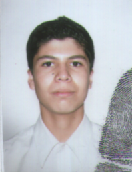
\includegraphics[scale=1]{foto_CV.png} }
&{\Large \textbf{Luis Miguel Pineda Daza}}

Licenciatura en Matemáticas Aplicadas y Computación 

Estudiante (octavo semestre)

\ 

{\large \textbf{Datos personales}}


\begin{tabular}{p{3cm} l}


\emph{Edad}&25 a\~nos\\

\emph{Tel\'efono} &55 25 01 77 41\\

\emph{E-mail}&
\textit{miguelpinedaza@gmail.com}\\

\emph{Direcci\'on}&Naucalpan, Estado de
Mex., CP 53270. \\



\end{tabular}
\end{tabular}
\\
\\
\\

\ 

\begin{minipage}[t]{0.45\textwidth}
	\vspace{-\baselineskip} % Required for vertically aligning minipages

\begin{large}
\textbf{Objetivos}
\end{large}


Obtener un puesto en el área  especifica  aplicando mis conocimientos adquiridos y contribuir astutamente en el beneficio de la empresa.

\end{minipage}
\hfill % Whitespace between
\begin{minipage}[t]{0.5\textwidth}
\begin{flushright}
	\vspace{-\baselineskip} % Required for vertically aligning minipages

\begin{large}
\textbf{Educación}
\end{large}


Licenciatura en 

Matemáticas Aplicadas y Computación

(octavo semestre)

Facultad de Estudios Superiores-Acatlán

\end{flushright}
\end{minipage}



\begin{comment}
Perfil del profesionista

El licenciado en Matemáticas Aplicadas y Computación es un profesionista capaz de utilizar las matemáticas y la computación de manera creativa para formular, analizar, diseñar, construir y automatizar soluciones a problemas reales. Durante su desempeño profesional ejercerá sus habilidades para actuar en equipos y adaptar métodos abstractos a la solución de problemas de orden práctico, así como a la modelación matemática y computacional de situaciones reales, con un pensamiento crítico, creativo e innovador de naturaleza inter y multidisciplinaria.

Estará capacitado para desempeñar actividades como:
Identificar problemas y proponer soluciones. Proponer constructos matemáticos-computacionales. Participar en equipos de investigación aplicada y documental en tecnologías de información, comunicación y desarrollo de software y hardware, para apoyar los procesos y servicios de una organización. Ofrecer consultoría en áreas físico-matemáticas y económico-administrativas, en inteligencia artificial, en tecnologías de la información, sistemas y programas de última generación. Atender las necesidades empresariales a través de la capacitación o actualización académicas. Desarrollar y manejar software: de sistema, de aplicación para resolver necesidades específicas de negocio, científico, empotrado, de línea de producto, así como aplicaciones de inteligencia artificial basadas en la Web y dispositivos móviles. Desempeñar la docencia en niveles de pregrado.
Objetivo

Desarrollar en el alumno la capacidad de aplicar creativamente las matemáticas y técnicas computacionales para analizar, evaluar y resolver problemas por medio de modelos en diversas áreas de conocimiento.
Características y habilidades recomendables del estudiante

El estudiante de Matemáticas Aplicadas y Computación debe poseer los conocimientos necesarios del área físico-matemática, contar con facilidad y razonamiento lógico, capacidad de concentración, de análisis y síntesis; tener una gran creatividad y curiosidad científica, así como de disciplina y constancia en el estudio y habilidad para el trabajo en equipo.
\end{comment}


\ 

%El esfuerzo de mi trabajo debe estar en proporci\'on a mi salario.






%Enfocado en la soluci\'on de problemas mediante modelos matem\'aticos y computaci\'on con el uso de las tecnolog\'ias emergentes, interactuando con diferentes \'areas del conocimiento y disciplinas.

\ 

\begin{large}
\textbf{Conocimiento}
\end{large}

\ 

Experiencia en la plataforma de eCommerce MAGENTO, realizando customizaciones de archivos  css / xml / phtml / js así mismo la creación de módulos y extensiones.

\ 

Manejo de shell en los sistemas operativos Unix y Windows.

\ 

Conocimiento de lenguajes de programación: C, C++,  SQL, Python, Java, JavaScript, Html5, PHP y CSS, y manejo de Office (excel avanzado). 

\ 

Realice mi servicio social en el Programa de Apoyo a Proyectos para la Innovación y Mejoramiento de la Enseñanza (PAPIME), realizando un Taller De Mantenimiento y Soporte T\'ecnico %con el tema de Instalaci\'on y Configuraci\'on de un Sistema Operativo 
con el Dr. Eduardo Eloy Loza Pacheco.


\ 

\begin{large}
\textbf{Experiencia Laboral}
\end{large}

\ 

\begin{tabular}{l p{12cm}}

\multirow{3}{3cm}{2019-11/2020-3 }
&

\textbf{doto.com.mx}  Desarrollador.

Mantenimiento de la pagina web doto.com.mx desarrollando back-end y front-end.
\\
&\\

\multirow{3}{3cm}{2019-8/2019-9 }
&
\textbf{Promociones y Display Marketing.} Sistemas y Soporte.


Manejo de base de datos, generando reportes y altas de eventos, asignación de usuarios y contraseñas.
\\
&\\

\multirow{2}{3cm}{2016-6/2016-8 \\2017-6/2017-8 }
&

\textbf{McDonald's, Naucalapan, Méx.}
Empleado General
 


Conocimiento en cocina y atención al cliente.
\\
&\\

\multirow{2}{3cm}{2016-11/2017-1}
&

\textbf{Empacador de pan, MEGA San Mateo.}
Empleado general


Elaboración del producto y atención al cliente
\\
&\\
\multirow{3}{3cm}{2015-2/2015-9}
&
\textbf{Burger King M\'exico - Naucalpan, M\'ex. 
}Líder de producción

Manejo de tiempos y temperaturas de la producción del producto así como la evaluación de empleados.

\end{tabular}



\begin{large}
\textbf{Logros}
\end{large}


\ 

Diploma especial por reconocimiento a la labor de excelencia operativa en Burger King México.

\ 

Reconocimiento por haber impartido la ponencia ``La forma canónica local''  dentro del ``Seminario de Geometría Diferencial de Curvas y Superficies''  realizado en la Facultad de Estudios Superiores - Acatlán.



\end{document}